\hypertarget{matdata_8h}{
\section{matdata.h File Reference}
\label{matdata_8h}\index{matdata.h@{matdata.h}}
}


This graph shows which files directly or indirectly include this file:\begin{figure}[H]
\begin{center}
\leavevmode
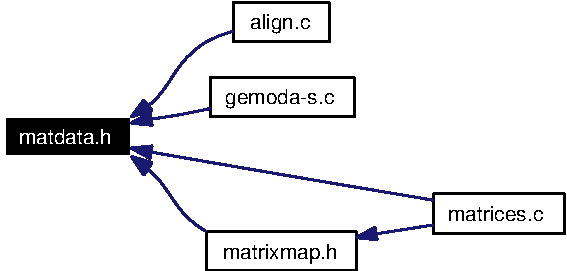
\includegraphics[width=153pt]{matdata_8h__dep__incl}
\end{center}
\end{figure}
\subsection*{Defines}
\begin{CompactItemize}
\item 
\#define \hyperlink{matdata_8h_a0}{MATRIX\_\-SIZE}~23
\end{CompactItemize}


\subsection*{Detailed Description}
This file defines the size of the scoring matrices so that we don't have to pound-include the whole \hyperlink{matrices_8h}{matrices.h} file due to worries about incompatibilities with earlier extern variable declarations.

Definition in file \hyperlink{matdata_8h-source}{matdata.h}.

\subsection*{Define Documentation}
\hypertarget{matdata_8h_a0}{
\index{matdata.h@{matdata.h}!MATRIX_SIZE@{MATRIX\_\-SIZE}}
\index{MATRIX_SIZE@{MATRIX\_\-SIZE}!matdata.h@{matdata.h}}
\subsubsection[MATRIX\_\-SIZE]{\setlength{\rightskip}{0pt plus 5cm}\#define MATRIX\_\-SIZE~23}}
\label{matdata_8h_a0}




Definition at line 10 of file matdata.h.

Referenced by main().
